\documentclass[svgnames, aspectratio = 1610]{beamer}
\linespread{1.2}
\usepackage[compatibility = false]{caption}
\usepackage{graphicx, subcaption, array, booktabs, mathtools, extarrows,
            tikz, mhchem, physics2, fixdif, derivative, lmodern, dsfont,
            CJKutf8, url, paracol, microtype, bm, ragged2e, multicol, menukeys}
\usepackage[mono = false]{libertine}
\DeclareRobustCommand \iu {\mathrm i\mkern1mu}
\DeclareMathOperator \upe {e}
\usetheme{westlake}
\justifying
\usepackage{zref-clever, zref-titleref}
\setlength \abovedisplayskip {6pt}
\setlength \belowdisplayskip {6pt}
\graphicspath{{./media/}}

\westlakeset{
  title      = Band Structure of 2D Kagome Lattice,
  subtitle   = Presentation of \textsf{Advanced Quantum Mechanics},
  author     ={ \texorpdfstring{Mingyu Xia (夏明宇) |
                \textit{Department of Physics, Westlake University}}%
                  {Mingyu Xia}, Mingyu Xia},
  date       = {\texttt{2026-01-09 \textbar\ E10-215@Yungu Campus}},
  background = bgimage,
  bibsource  = reference.bib,
}

\begin{document}

\begin{CJK*}{UTF8}{gbsn}
\maketitle
\end{CJK*}

\section{INTRODUCTION}

\begin{frame}{What is Kagome? --- The Trihexagonal}
  \begin{block}{Coined by Kôdi Husimi}
    \begin{columns}
    \begin{column}{.72\linewidth}
      The kagome lattice first appeared in a paper by Kôdi Husimi's assistant
      Ichirō Shōji~\cite{WikipediA}. Satisfying the \texttt{p6m} symmetry.
      \begin{itemize}
        \item Six-fold rotation about hexagon centers
        \item Multiple mirror reflection lines
        \item Triangular and hexagonal sublattice symmetries
        \item Combined rotation-reflection ($C_6\sigma$) operations
      \end{itemize}
    \end{column}
    \hfill
    \begin{column}{.24\linewidth}
      \centering
      \includegraphics[width = \linewidth]{Tiling_3-6_simple.svg.png}
    \end{column}
    \end{columns}
  \end{block}
  \pause
  \begin{exampleblock}{Outlook}
    \begin{itemize}
      \item Discovering new Kagome materials
      \item Kagome quantum spin liquid and superconducting behaviors
      \item Kagome topological properties
    \end{itemize}
  \end{exampleblock}
\end{frame}

\begin{frame}{Lattice Structure}
  \begin{block}{Three type of sites}
    \begin{itemize}
      \item Marked as \textcolor{blue}{$A$ (blue)}, \textcolor{red}{$B$ (red)},
      and \textcolor{Green}{$C$ (green)}, respectively
      \item Hops' magnitude between different type of sites are different
    \end{itemize}
  \end{block}
  \begin{figure}[htbp]
    \begin{minipage}[t]{.48\linewidth}
      \centering
      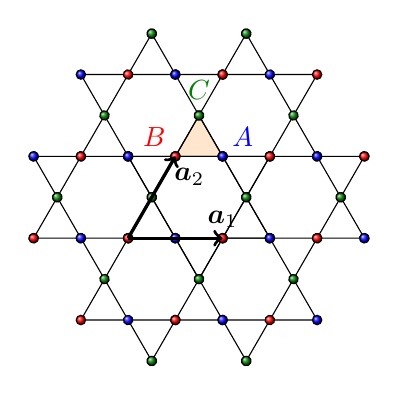
\begin{tikzpicture}[scale = .6]
        \fill [orange, opacity = .2]
          (.5,{sqrt(3)}) node [opacity = 1, blue, above right] {$A$} --++
          (-1,0) node [opacity = 1, red, above left] {$B$} --++
          (60:1) node [opacity = 1, Green, above = .5ex] {$C$} -- cycle;
        \foreach \i in {0, 180}
          {
        \begin{scope}[rotate around = {\i:(0,{sqrt(3)/2})}]
          \draw (-3.5,0) --++ (5,0) --++ (120:5) --++ (240:5) -- cycle;
          \draw (-1.5,0) --++ (5,0) --++ (120:5) --++ (240:5) -- cycle;
          \draw (-2.5,{-sqrt(3)}) --++ (5,0) --++ (120:5) --++ (240:5) -- cycle;
        \end{scope}
          }
        \foreach \i in {0, 180}
          {
        \begin{scope}[rotate around = {\i:(0,{sqrt(3)/2})}]
          \foreach \j in {0, 2}
          {
        \begin{scope}[xshift = \j cm]
          \shade [draw, ball color = blue] (-2.5,0) circle (.1);
          \shade [draw, ball color = blue] (-.5,0) circle (.1);
          \shade [draw, ball color = blue] (1.5,0) circle (.1);
          \shade [draw, ball color = red] (-3.5,0) circle (.1);
          \shade [draw, ball color = red] (-1.5,0) circle (.1);
          \shade [draw, ball color = red] (.5,0) circle (.1);
          \begin{scope}[rotate around = {60:(-3.5,0)}]
            \shade [draw, ball color = red] (-3.5,0) circle (.1);
            \shade [draw, ball color = red] (-1.5,0) circle (.1);
            \shade [draw, ball color = red] (.5,0) circle (.1);
            \shade [draw, ball color = Green] (-2.5,0) circle (.1);
            \shade [draw, ball color = Green] (-.5,0) circle (.1);
            \shade [draw, ball color = Green] (1.5,0) circle (.1);
          \end{scope}
          \begin{scope}[rotate around = {-60:(1.5,0)}]
            \shade [draw, ball color = Green] (-3.5,0) circle (.1);
            \shade [draw, ball color = Green] (-1.5,0) circle (.1);
            \shade [draw, ball color = Green] (.5,0) circle (.1);
            \shade [draw, ball color = blue] (-2.5,0) circle (.1);
            \shade [draw, ball color = blue] (-.5,0) circle (.1);
            \shade [draw, ball color = blue] (1.5,0) circle (.1);
          \end{scope}
          \shade [draw, ball color = red] (-2.5,{-sqrt(3)}) circle (.1);
          \shade [draw, ball color = blue] (.5,{-sqrt(3)}) circle (.1);
        \end{scope}
          }
        \end{scope}
          }
        \draw [very thick, ->] (-1.5,0) --++ (2,0)
         node [above] {$\bm a_1$};
        \draw [very thick, ->] (-1.5,0) --++ (60:2)
         node [near end, right] {$\bm a_2$};
      \end{tikzpicture}
    \end{minipage}
    \hfill
    \begin{minipage}[t]{.48\linewidth}
      \centering
      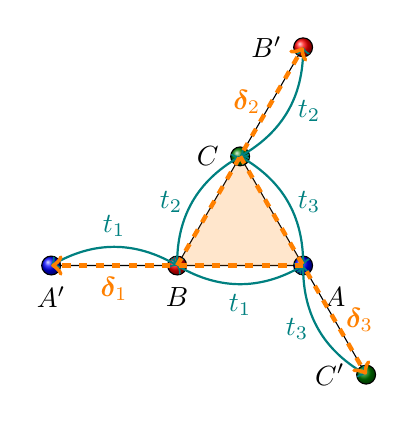
\begin{tikzpicture}[scale = .8]
        \draw (2,0) -- (-2,0)
              (0,0) -- (2,{2*sqrt(3)})
              (1,{sqrt(3)}) -- (3,{-sqrt(3)});
        \fill [orange, opacity = .2] (0,0) -- (1,{sqrt(3)}) -- (2,0) -- cycle;
        \shade [draw, ball color = blue] (2,0) circle (.15) coordinate (A)
         node [below right = .15cm] {$A$};
        \shade [draw, ball color = red] (0,0) circle (.15) coordinate (B)
         node [below = .15cm] {$B$};
        \shade [draw, ball color = Green] (1,{sqrt(3)}) circle (.15)
         coordinate (C) node [left = .15cm] {$C$};
        \shade [draw, ball color = blue] (-2,0) circle (.15)
         coordinate (A') node [below = .15cm] {$A'$};
        \shade [draw, ball color = red] (2,{2*sqrt(3)}) circle (.15)
         coordinate (B') node [left = .15cm] {$B'$};
        \shade [draw, ball color = Green] (3,{-sqrt(3)}) circle (.15)
         coordinate (C') node [left = .15cm] {$C'$};
        \draw [thick, <->, teal] (A) to[bend left] node [below] {$t_1$} (B);
        \draw [thick, <->, teal] (B) to[bend left] node [left] {$t_2$} (C);
        \draw [thick, <->, teal] (C) to[bend left] node [right] {$t_3$} (A);
        \draw [thick, <->, teal] (B) to[bend right] node [above] {$t_1$} (A');
        \draw [thick, <->, teal] (C) to[bend right] node [right] {$t_2$} (B');
        \draw [thick, <->, teal] (A) to[bend right] node [left] {$t_3$} (C');
        \draw [ultra thick, dashed, ->, orange] (B) --
         node [left, near end] {$\bm \delta_2$} (B');
        \draw [ultra thick, dashed, ->, orange] (A) --
         node [below, near end] {$\bm \delta_1$} (A');
        \draw [ultra thick, dashed, ->, orange] (C) --
         node [right, near end] {$\bm \delta_3$} (C');
      \end{tikzpicture}
    \end{minipage}
    \caption{Top view of the Kagome Lattice and
      tight-binding model with NN hopping}
    \zlabel{fig:Kagome}
  \end{figure}
\end{frame}

\section{METHODOLOGY}

\begin{frame}{Model Hamiltonian}
  \begin{alertblock}{Tight-binding model in second
    quantization~\cite{PhysRevB.102.045151}}
    Consider the nearest-neighbor (NN) hopping
    \begin{equation}
      \mathcal H = -\sum_{\bm r}[
        t_1(\hat a_{\bm r}^\dagger \hat b_{\bm r}
        + \hat b_{\bm r}^\dagger \hat a_{\bm r+\bm\delta_1})
        + t_2(\hat b_{\bm r}^\dagger \hat c_{\bm r}
        + \hat c_{\bm r}^\dagger \hat b_{\bm r+\bm\delta_2})
        + t_3(\hat c_{\bm r}^\dagger \hat a_{\bm r}
        + \hat a_{\bm r}^\dagger \hat c_{\bm r+\bm\delta_3})]
        + \text{H.c.}
      \label{eq:Hamiltonian_NN}
    \end{equation}
    The operators $\hat a_{\bm r}$ ($\hat a_{\bm r}^\dagger$),
    $\hat b_{\bm r}$ ($\hat b_{\bm r}^\dagger$),
    $\hat c_{\bm r}$ ($\hat c_{\bm r}^\dagger$)
    stands for annihilating (or creating) an electron at site $\bm r$.
  \end{alertblock}
  \pause
  \begin{block}{Uniform labels via Fourier transformation}
    Raising an extra phase factor for the annihilation/creation operators of
    the NN sites
    \[
      \hat o_{\bm r+\bm\delta_i} = \frac1{\sqrt N} \sum_{\bm k}
        \upe^{\iu\bm k(\cdot\bm r+\bm\delta_i)} \hat o_{\bm k}, \quad
      \hat o_{\bm r+\bm\delta_i}^\dagger = \frac1{\sqrt N} \sum_{\bm k}
        \upe^{-\iu\bm k(\cdot\bm r+\bm\delta_i)} \hat o_{\bm k}
    \]
    Operators $\hat o = \{\hat a, \hat b, \hat c\}$.
  \end{block}
\end{frame}

\begin{frame}{Dispersion Relation}
  \begin{block}{Diagonalized Hamiltonian}
    \begin{equation}
      \mathcal H
    = \sum_{\bm k} \Psi_{\bm k}^\dagger \tilde{\mathcal H} \Psi_{\bm k}
    = \sum_{\bm k}
      \begin{pmatrix}
        \hat a_{\bm k}^\dagger\\ \hat b_{\bm k}^\dagger\\ \hat c_{\bm k}^\dagger
      \end{pmatrix}^{\mkern-1.5mu\mathsf T}
      \begin{pmatrix}
        0 & -t_1(1 + \upe^{-\iu\bm k\cdot\bm\delta_1})
          & -t_3(1 + \upe^{+\iu\bm k\cdot\bm\delta_3})\\
            -t_1(1 + \upe^{+\iu\bm k\cdot\bm\delta_1}) & 0
          & -t_2(1 + \upe^{-\iu\bm k\cdot\bm\delta_2})\\
            -t_3(1 + \upe^{-\iu\bm k\cdot\bm\delta_3}) &
            -t_2(1 + \upe^{+\iu\bm k\cdot\bm\delta_2}) & 0
      \end{pmatrix}
      \begin{pmatrix}
        \hat a_{\bm k}\\ \hat b_{\bm k}\\ \hat c_{\bm k}
      \end{pmatrix}
      \label{eq:diagonalized_Hamiltonian}
    \end{equation}
  \end{block}
  \pause
  \begin{exampleblock}{Eigen Equation}
    From $\det(\tilde{\mathcal H} - E\mathds 1) = 0$, one
    can obtain a cubic polynomial in $E$
    \begin{equation}
      E^3 - 2E \sum_i^3 t_i^2 (1 + \cos(\bm k \cdot \bm\delta_i))
      + 4t_1t_2t_3 \ab[1 + \sum_i^3 \cos(\bm k \cdot \bm\delta_i)] = 0
      \label{eq:dispersion_relation_expand}
    \end{equation}
    This is a universal result.
  \end{exampleblock}
  \pause
  \begin{alertblock}{}\centering \Large
    \menu[,]{Cubic eigen equation, Three energy bands} =
    \menu{Two dispersive bands} + \menu{One flat band}
  \end{alertblock}
\end{frame}

\section{RESULT DISCUSSION}

\begin{frame}{Band Structure}
  \begin{block}{Trivial case}
    Simply taking $t_1 = t_2 = t_3 = t$
    \begin{equation}
      E_\pm
    = t\ab[-1 \pm \sqrt{\textstyle 3 + 2\sum_i^3
      \cos(\bm k \cdot \bm\delta_i)}], \quad
      E_\text{flat} = 2t
      \label{eq:band}
    \end{equation}
  \end{block}
  \pause
  \begin{exampleblock}{Numerical plotting}
    \begin{figure}[htbp]
      \begin{minipage}{.22\linewidth}
        \centering
        \includegraphics[page = 1, height = .32\paperheight]{kagome_bands.pdf}
      \end{minipage}
      \hfill
      \begin{minipage}{.22\linewidth}
        \centering
        \includegraphics[page = 2, height = .32\paperheight]{kagome_bands.pdf}
      \end{minipage}
      \hfill
      \begin{minipage}{.26\linewidth}
        \centering
        \includegraphics[page = 3, height = .32\paperheight]{kagome_bands.pdf}
      \end{minipage}
      \hfill
      \begin{minipage}{.26\linewidth}
        \centering
        \includegraphics[page = 4, height = .32\paperheight]{kagome_bands.pdf}
      \end{minipage}
      \caption{3D/2D Band structure for NN hopping under different perspectives
        plotted by \textsf{Python}}
      \zlabel{fig:3Dband}
    \end{figure}
  \end{exampleblock}
\end{frame}

\begin{frame}{Dirac Point}
  \begin{exampleblock}{At the Dirac point}
  \begin{columns}
  \begin{column}{.72\linewidth}
    Taking $K = \frac{2\pi}{a}\ab(0, \frac1{\sqrt3})$
    \[
      E_+ = 2t = E_\text{flat},\quad E_- = -4t
    \]
    Implies that $E_\text{flat}$ and $E_+$ are tangent at four $K$-points,
    which can be seen in the right figure.
  \end{column}
  \hfill
  \begin{column}{.24\linewidth}
    \centering
    \includegraphics[page = 2, width = \linewidth]{kagome_bands.pdf}
  \end{column}
  \end{columns}
  \end{exampleblock}
  \pause
  \begin{block}{Near the Dirac point}
    Taking $\bm k = \bm b_2 + \bm q$ with $|\bm q| \ll 1$
    \[
      E_+ = t\ab(2 - \frac43\pi^2|\bm q^2|),\quad
      E_- = t\ab(-4 + \frac43\pi^2|\bm q|^2)
    \]
    Indicates that the dispersive bands around the Dirac points are parabolic.
  \end{block}
\end{frame}

\section{ADVANCED STUDY}

\begin{frame}{An Extra NNN or NNNN Hopping}
  \visible<1->{%
  The Hamiltonian with the NNN or NNNN hopping term
  \begin{equation}
    \mathcal H' = \mathcal H_\text{NN}(t_i') + \mathcal H_\text{NNN/NNNN}(t_i'')
  \end{equation}}%
  \vspace{-9pt}
  \begin{columns}
    \begin{column}{.6\linewidth}
      \visible<3->{%
      with the corresponding diagonalized ones
      \begin{align}
        \mathcal H_\text{NNN} & = -\sum_{\bm r}[t_1'(
          \hat a_{\bm r}^\dagger \hat b_{\bm r+\bm\delta_2}
        + \hat b_{\bm r}^\dagger \hat c_{\bm r+\bm\delta_3}
        + \hat c_{\bm r}^\dagger \hat a_{\bm r+\bm\delta_1})] + \text{H.c.}
        \notag\\
    & = \sum_{\bm k}
        \Psi_{\bm k}^\dagger
        \begin{psmallmatrix}
          0 & -t_1'\upe^{+\iu\bm k\cdot\bm\delta_2} &
              -t_3'\upe^{-\iu\bm k\cdot\bm\delta_1}\\
              -t_1'\upe^{-\iu\bm k\cdot\bm\delta_2} & 0 &
              -t_2'\upe^{+\iu\bm k\cdot\bm\delta_3}\\
              -t_3'\upe^{+\iu\bm k\cdot\bm\delta_1} &
              -t_2'\upe^{-\iu\bm k\cdot\bm\delta_3} & 0
        \end{psmallmatrix}
        \Psi_{\bm k}\\
        \mathcal H_\text{NNNN} & = -\sum_{\bm r}[
          t_1'' \hat a_{\bm r}^\dagger \hat a_{\bm r+\bm\delta_1}
        + t_2'' \hat b_{\bm r}^\dagger \hat b_{\bm r+\bm\delta_2}
        + t_3'' \hat c_{\bm r}^\dagger \hat c_{\bm r+\bm\delta_3}]
        + \text{H.c.}\notag\\
        & =
        \begin{psmallmatrix}
          -2t_1''\cos(\bm k \cdot \bm \delta_1)\\
        & -2t_2''\cos(\bm k \cdot \bm \delta_2)\\
      & & -2t_3''\cos(\bm k \cdot \bm \delta_3)
        \end{psmallmatrix}
      \end{align}}%
    \end{column}
    \hfill
    \visible<2->{%
    \begin{column}{.36\linewidth}
      \begin{figure}[htbp]
        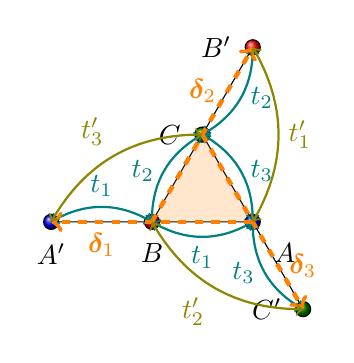
\begin{tikzpicture}[scale = .64]
          \draw (2,0) -- (-2,0)
                (0,0) -- (2,{2*sqrt(3)})
                (1,{sqrt(3)}) -- (3,{-sqrt(3)});
          \fill [orange, opacity = .2] (0,0) -- (1,{sqrt(3)}) -- (2,0) -- cycle;
          \shade [draw, ball color = blue] (2,0) circle (.15) coordinate (A)
           node [below right = .15cm] {$A$};
          \shade [draw, ball color = red] (0,0) circle (.15) coordinate (B)
           node [below = .15cm] {$B$};
          \shade [draw, ball color = Green] (1,{sqrt(3)}) circle (.15)
           coordinate (C) node [left = .15cm] {$C$};
          \shade [draw, ball color = blue] (-2,0) circle (.15)
           coordinate (A') node [below = .15cm] {$A'$};
          \shade [draw, ball color = red] (2,{2*sqrt(3)}) circle (.15)
           coordinate (B') node [left = .15cm] {$B'$};
          \shade [draw, ball color = Green] (3,{-sqrt(3)}) circle (.15)
           coordinate (C') node [left = .15cm] {$C'$};
          \draw [thick, <->, teal] (A) to[bend left] node [below] {$t_1$} (B);
          \draw [thick, <->, teal] (B) to[bend left] node [left] {$t_2$} (C);
          \draw [thick, <->, teal] (C) to[bend left] node [right] {$t_3$} (A);
          \draw [thick, <->, teal] (B) to[bend right] node [above] {$t_1$} (A');
          \draw [thick, <->, teal] (C) to[bend right] node [right] {$t_2$} (B');
          \draw [thick, <->, teal] (A) to[bend right] node [left] {$t_3$} (C');
          \draw [ultra thick, dashed, ->, orange] (B) --
           node [left, near end] {$\bm \delta_2$} (B');
          \draw [ultra thick, dashed, ->, orange] (A) --
           node [below, near end] {$\bm \delta_1$} (A');
          \draw [ultra thick, dashed, ->, orange] (C) --
           node [right, near end] {$\bm \delta_3$} (C');
          \draw [thick, <->, olive] (A) to[bend right]
           node [right] {$t_1'$} (B');
          \draw [thick, <->, olive] (B) to[bend right]
           node [below left] {$t_2'$} (C');
          \draw [thick, <->, olive] (C) to[bend right]
           node [above left] {$t_3'$} (A');
        \end{tikzpicture}
        \caption{Graph for NN and NNN hopping}
        \zlabel{fig:NNN_splice}
      \end{figure}
    \end{column}}%
  \end{columns}
  \visible<4->{%
  Interesting, $\mathcal H_\text{NNNN}$ is a diagonal matrix. Energy bands can
  be obtained from $\det(\tilde{\mathcal H} - E\mathds 1) = 0$.}%
\end{frame}

\nocite{*}
\printbibliography

\section{Thanks for Listening! Any Questions?}

\end{document}
